\subsubsection{i)}
This Exercise has been completed in the attached Jupyter Notebook titled: "integration".\\
The resulting plot is given here:\\
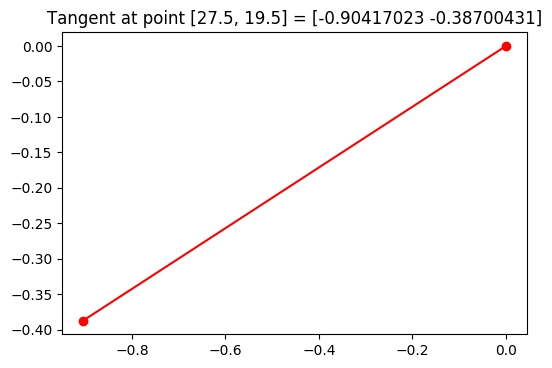
\includegraphics[width=0.75\linewidth]{tanpoint2820}\\
The most crucial part of the code is the following, which simply rounds the values given and returns the tangent in the given point:
\begin{verbatim}
def tanDir(floatPos, tanArr):
    intx = int(round(floatPos[0]))
    inty = int(round(floatPos[1]))
    return tanArr[intx,inty]
\end{verbatim}
\subsubsection{ii)}
The coding part of this Exercise has been completed in the attached Jupyter Notebook titled: "integration". \\
When plotting the euler function on top of the tangential directions, you will see that the function follows the direction of the "flow". This means that in places where the vectors are all long and in a similar direction, the function will go fast in that direction, such as in the starting point $[28,20]$. On the other hand, starting somewhere like $[12,16]$, the vectors are all short and their direction seems at least sort of random, so each step will be short, and in an unpredictable direction.
The resulting plot is given here: \\
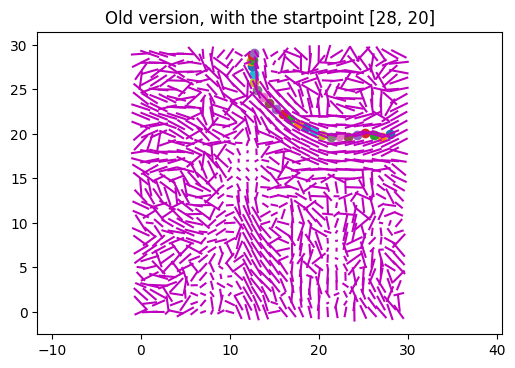
\includegraphics[width=0.75\linewidth]{old2820} \\
And the most crucial part of the code is the following, which creates a list of vectors, containing the coordinates for each step:
\begin{verbatim}
def euler(s, start, length, array):
    curPos = start.copy()
    retVal = [curPos]
    
    for i in range(length):
        # Checking if curPos is inside the given dataset
        if (curPos[0] < len(array)-1 and curPos[1] < len(array)-1 and curPos[0] > 0 and curPos[1] > 0):
            # Updating curPos with the tangents direction in the given point
            curPos += tanDir(curPos,array)
            retVal.append(curPos.copy())
        else:
            # Breaking out of the loop
            i = length
    return retVal
\end{verbatim}

\subsubsection{iii)}
The coding part of this Exercise has been completed in the attached Jupyter Notebook titled: "integration". \\
To calculate which step would result in the smallest change in direction, you first have to figure out whether you came to this point via an inverted vector, if you did, you make sure that the vector you are reading for the current position is inverted as well. Then, you figure out whether the next vector should be inverted. This is done with some linear algebra, by calculating the angle between the current vector and the next vector in line. If the next vector should be inverted, we set a flag to make sure we invert it, as we checked for in the beginning. Then, we simply add the current vector the out current position.\\
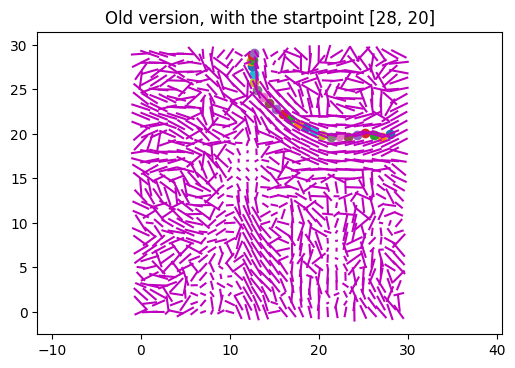
\includegraphics[width=0.5\linewidth]{old2820}
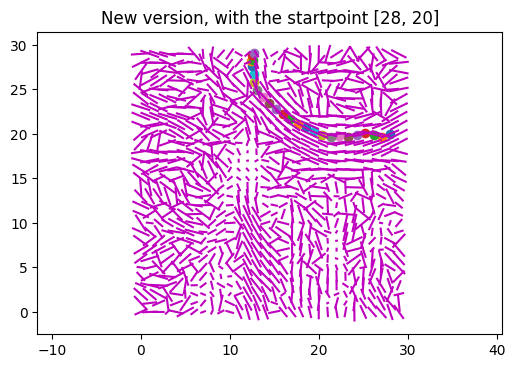
\includegraphics[width=0.5\linewidth]{new2820}
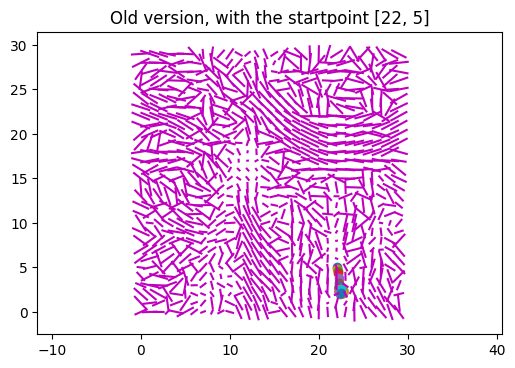
\includegraphics[width=0.5\linewidth]{old225}
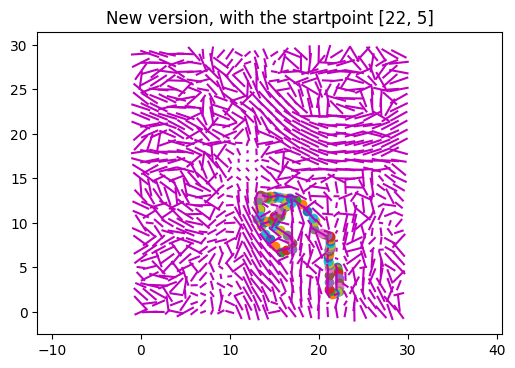
\includegraphics[width=0.5\linewidth]{new225}
The code for this bit has changed significantly, to take into account whether both the current, and the next vector is negative:
\begin{verbatim}
def newEuler(s, start, length, array):
    curPos = start.copy()
    retVal = [curPos]
    wasMinus = False
    for i in range(length):
        # Checking if curPos is inside the given dataset
        if (curPos[0] < len(array)-1 and curPos[1] < len(array)-1 and curPos[0] > 0 and curPos[1] > 0):
            
            # Determining which direction next step is
            if (wasMinus):
                curVec = -tanDir(curPos.copy(),array)
            else:
                curVec = tanDir(curPos.copy(),array)
            plusVector = tanDir((curPos.copy()+curVec),array)
            minusVector = -tanDir((curPos.copy()+curVec),array)
            # Updating curPos with the tangents direction in the given point
            if (vectorAngle(curVec,plusVector) < vectorAngle(curVec,minusVector)):
                wasMinus = False
            else:
                wasMinus = True
            
            curPos += curVec
            retVal.append(curPos.copy())
        else:
            # Breaking out of the loop
            i = length +1
    return retVal
\end{verbatim}
\subsubsection{iv)}
One thing that stand out, seems to be the fact that plotting these tangents takes a surprisingly long time, even for a dataset as small as this one. With larger datasets, it would seem that this could be a problem.\\
Another problem with using the euler method is that while you can see where a fiber leads/comes from, from just a single element, you can only see it in one  direction, that is, you cannot see where it would go further. Perhaps this could be fixed with an opposite function that instead of calculating for the positive value of the vector in the starting position, it would calculate for the negative value.